%!TEX TS-program = xelatex
\documentclass[]{friggeri-cv}
\usepackage{afterpage}
\usepackage{hyperref}
\usepackage{color}
\usepackage{xcolor}
\hypersetup{
    pdftitle={},
    pdfauthor={},
    pdfsubject={},
    pdfkeywords={},
    colorlinks=false,       % no lik border color
   allbordercolors=white    % white border color for all
}
\addbibresource{bibliography.bib}
\RequirePackage{xcolor}
\definecolor{pblue}{HTML}{0395DE}

\begin{document}
\header{FranciscoIvan}{RodriguezLopez}
      {Desarrollador web}
      
% Fake text to add separator      
\fcolorbox{white}{gray}{\parbox{\dimexpr\textwidth-2\fboxsep-2\fboxrule}{%
.....
}}

% In the aside, each new line forces a line break
\begin{aside}
  \begin{figure}
    %\hfill
    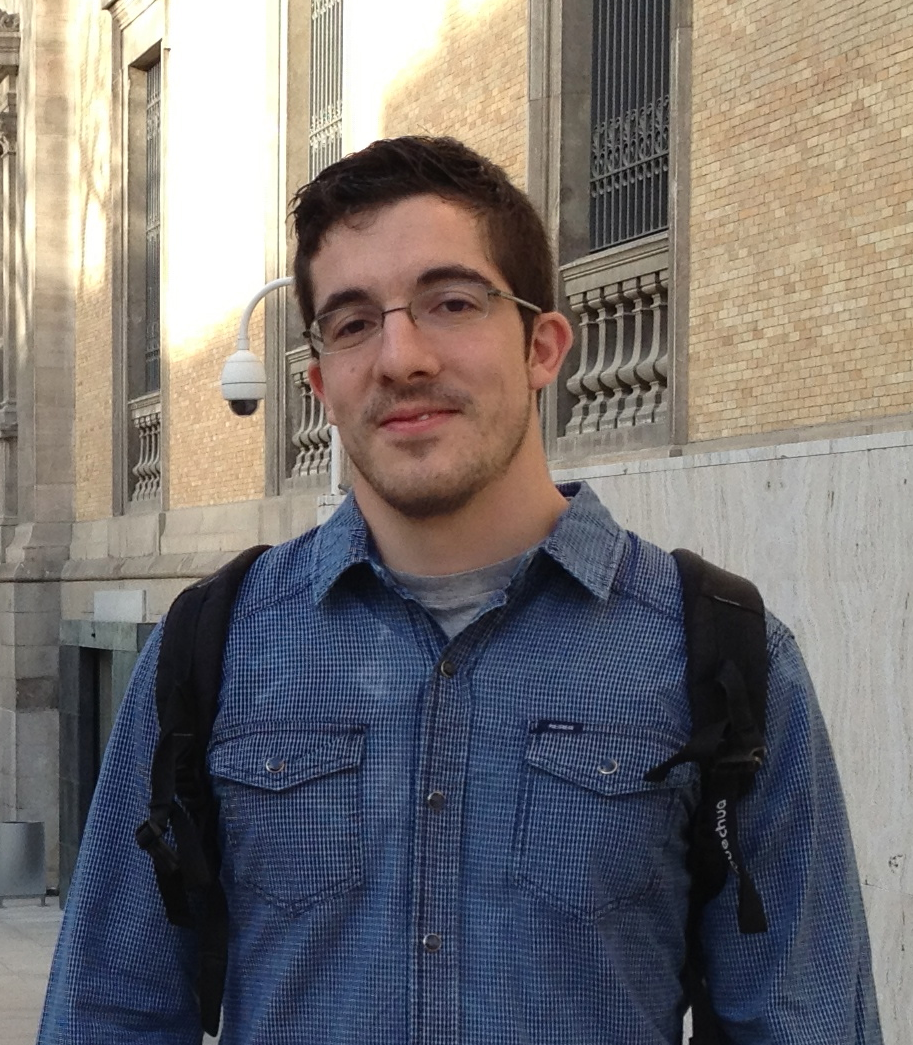
\includegraphics[width=0.6\columnwidth]{foto.png}
    %\vspace{-7cm}
  \end{figure}
  
  % \section{Address}
  %   Arroyo de la Media Legua, 1
  %   Madrid, Spain
  %   ~
  \section{Tel}% \& Skype}
   ~
    +34 620 38 00 27
    ~
  \section{Mail}
    \href{mailto:frivanrodriguez@gmail.com}{\textbf{frivanrodriguez@}\\gmail.com}
    ~
  \section{LinkedIn \& Git}
    \href{es.linkedin.com/pub/francisco-iván-rodríguez-lópez/}{linkedin.com/francisco-iván-rodríguez-lópez/}
    \href{https://github.com/ivanrod}{github.com/ivanrod}
    ~
  \section{Programación}
    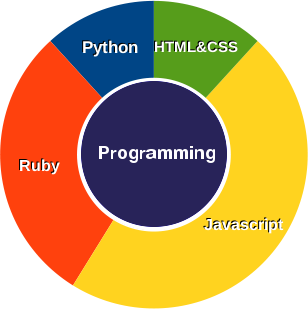
\includegraphics[scale=0.50]{img/programming2.png}
    ~
  \section{SO Preferidos}
    \textbf{GNU/Linux}
\includegraphics[scale=0.40]{img/5stars.png}
    \textbf{Windows}
\includegraphics[scale=0.40]{img/4stars.png}
    ~
  \section{Habilidades personales}
    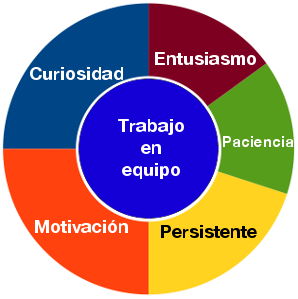
\includegraphics[scale=0.50]{img/softSkills.png}
    ~
  %\section{Places Lived}
  %  \includegraphics[scale=0.25]{img/italia.png}
  %  ~
  \section{Idiomas}
    \textbf{Español}
\includegraphics[scale=0.40]{img/5stars.png}
    \textbf{Portugués}
\includegraphics[scale=0.40]{img/4stars.png}
    \textbf{Inglés}
\includegraphics[scale=0.40]{img/3stars.png}
\end{aside}

\section{Intereses}

Javascript, AngularJS, NodeJS, Ruby, Python, GIS, Geolocalización, Big data, Visión artificial, Modelización 3D

\section{Resumen}
Ingeniero en geomática y cartografía, con solida formación en programación, buscando nuevos proyectos que me permitan crecer profesionalmente como desarrollador web
% %seeking a career position

% \textbf{GitHub:}\par
%     \href{url:https://github.com/ivanrod}{https://github.com/ivanrod}\par
% \textbf{LinkedIn:}\par
%     \href{url:es.linkedin.com/pub/francisco-iván-rodríguez-lópez/}{es.linkedin.com/pub/francisco-iván-rodríguez-lópez/}


\section{Educación}

\begin{entrylist}
  \entry
    {2014}
    {Programa Generation }%{\normalfont candidate in Computer Science}}
    {Ironhack. McKinsey Social Iniciative}
    {\emph{Desarrollo web orientado a la experiencia de usuario.} \par Tecnologías: HTML/CSS, JavaScript, Ruby, Ruby on Rails, Sinatra}
  \entry    
    {2011 - 2014}
    {Máster Oficial}%{\normalfont candidate in Computer Science}}
    {Universidad Politécnica de Madrid (UPM)}
    {\emph{Ingeniería Geodésica y Cartográfica (120 Créditos ECTS)}}
  \entry
    {2004 - 2009}
    {Ingeniería Técnica}
    {Universidad de Santiago de Compostela (USC)}
    {Topografía}
  \entry
    {2008–2009}
    {beca de intercambio}
    {Universidad del País Vasco (UPV/EHU)}
    {Programa SICUE/SENECA. Ing. Téc. en Topografía}
  \entry
    {2007–2008}
    {beca de intercambio}
    {Faculdade de Ciencias da Universidade de Lisboa}
    {Programa SOCRATES/ERASMUS. Ing. Téc. en Topografía}
\end{entrylist}

\section{Experiencia}

\begin{entrylist}
  \entry
    {2015}
    {Altran Innovación S.L.}
    {Desarrollador web}
    {\emph{Desarrollo de aplicaciones web. Tecnologías: AngularJS, Java Spring, Foundation, Foundation for apps,...}}
\end{entrylist}

\begin{entrylist}
  \entry
    {2014}
    {eGeomapping}
    {Ingeniero en geomática}
    {\emph{Trabajos de modelización 3D}}
\end{entrylist}

\section{Cursos}

\begin{entrylist}
  \entry
    {2013}
    {University of Toronto}
    {\href{https://www.coursera.org/course/programming2}{Coursera}}
    {Learn to Program: Crafting Quality Code}
  \entry
    {2013}
    {MIT}
    {\href{https://courses.edx.org/courses/MITx/6.00x/2013_Spring/info}{edX}}
    {6.00x Introduction to Computer Science and Programming}
  \entry
    {2013}
    {Universidad Politécnica de Valencia}
    {\href{http://miriadax.net/web/dispositivos_moviles}{Miriada X}}
    {Dispositivos Móviles - aplicaciones a la ingeniería y la gestión del territorio}
\end{entrylist}

\section{Publicaciones}
Rodriguez Lopez, Francisco Ivan\\
\textbf{{\href{http://oa.upm.es/30703/}{Representación 3D de petroglifos: propuesta de metodología de modelización de los grabados del Valle de Tamanart, Marruecos}}}\\
\emph{Trabajo fin de máster, Madrid, España, Julio, 2014}
%%% This piece of code has been commented by Karol Kozioł due to biblatex errors. 
% 
%\printbibsection{article}{article in peer-reviewed journal}
%\begin{refsection}
%  \nocite{*}
%  \printbibliography[sorting=chronological, type=inproceedings, title={international peer-reviewed conferences/proceedings}, notkeyword={france}, heading=subbibliography]
%\end{refsection}
%\begin{refsection}
%  \nocite{*}
%  \printbibliography[sorting=chronological, type=inproceedings, title={local peer-reviewed conferences/proceedings}, keyword={france}, heading=subbibliography]
%\end{refsection}
%\printbibsection{misc}{other publications}
%\printbibsection{report}{research reports}

\end{document}
